\subsection{Detecting Malware which Sends Spam Email} \label{sec:sensor-spam}

It is common that botnets are used to send spam email.
Spam can be sent out at different rates.
Some worms like Storm and Rustock have been reported to send at lowish
rates of 20 and 33 emails/min, while others can be high, e.g. Srizbi's rate is
1800 emails/min \cite{john2009studying}. While 20 emails/min is probably too
high for humans, malware could also send at lower rates.
We remark that humans might also send email at high rate, e.g.
when using a script to send emails to a group of recipients such 
as a mailing list.

Our experiment is meant to show
spam detection is reliable when the monitor uses
data from external sensors.
We also experiment on
different modes of sending email, namely,
SMTP-based clients and also webmail clients.

%\subsubsection{Spam Detection Using the Framework}
%\label{subsubsec:spam-detectmethod}

To detect bots that send spam, using our modified CuSum detection, we apply the following rules: (i) when
the user is absent, any outgoing email flags a spamming activity; and
(ii) when the user is present, our detection algorithms are applied on the
number of emails sent. Essentially, if over $N$ emails are sent
within a time interval of length $t$, the algorithm flags it as
spamming activity, where $N$ and $t$ are the two tunable parameters and carries slightly different meanings in each detection algorithm.

The first rule relies on the fact that emails are usually directly
sent to the mail servers when the user performs ``send''
in the email client. Any scheduled
delay in delivery is based on the server itself. The actual value of
$N$ and $t$ in the second rule can be learned from the normal
traffic for each host.
Although the rules are simple, no matter how slow the spam rate
is, we can detect spam when the user is absent. So if a
stealthy spam program sends out only a single email at night,
this could slip out unnoticed by normal email rate based spam detection
while we would detect it.

Figure~\ref{fig:email} shows the typical email activity of a
user in a day. About 10 to 20 emails are sent daily.
It shows that our hypothesis that all emails are sent with the
user present is reasonable.

\begin{figure}[htb]
\begin{center}
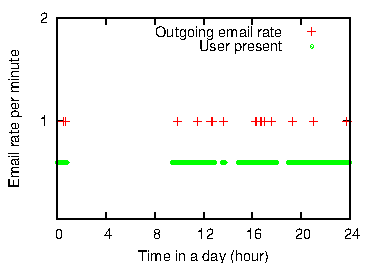
\includegraphics[width=0.6\textwidth]{sensor/email-norm}
\caption{Samples of user email rate}
\label{fig:email}
\end{center}
\end{figure}

When we apply CuSum to detect changes in the amount of emails sent when
the user is present, we incorporate a limit on the accumulation time
$t$, and set $a=0$, $N=120$ and $t=6$ hours. The effect is that
whenever there is an outgoing email, we accumulate the count, and no
more than $N=120$ emails can be sent in 6 hours. If the accumulated sum
exceeds 120, we raise a spam alarm for the host. The allowable
average email rate is three minutes per email. This is already high for a
human user, since users do not consistently send an email every 3
minutes for 6 hours. Using a lower threshold will make it even easier
to detect the spam.
When the user is absent, we set $N=1$, meaning any
outgoing email indicates that it is spam.

%\subsubsection{Experimental Results on Spammer Detection} \label{sec:spam-dect}

\begin{table}[!t]
  \centering
  \begin{tabular}{|c|c|c|}
  \hline
  Spam worm  & User present & User absent \\
  \hline
  Storm & 6.1 min & immediate \\
  \hline
  Rustock & 3.6 min & immediate \\
  \hline
  Srizbi & 5 sec & immediate \\ [0.5ex]
  \hline
  \end{tabular}
  \caption{Detection time of different spam worms. (Detection threshold $N=120$ emails in $t=6$ hours at user presence, and $N=1$ during user absence.)}
  \label{tbl:detect-spam}
\end{table}

In our experiment, spam is sent from the monitored host using the
modified Agobot.
We tested the detection of spam at rates corresponding to Srizbi,
Rustock and Storm worms.
We assume the spam emails are sent out at uniform rate.
Table~\ref{tbl:detect-spam} shows the
detection time when the user is present and absent.
Note that threshold $N$ is set on the parameter of the accumulated
email amount. It is easy to see the detection time is inversely
proportional to the spam rate. Since the spam rate of Srizbi is much
higher than Rustock or Storm, it takes least time to detect. When
the user is present, the detection time of Srizbi is within 5 seconds
and about 4 and 6 minutes for Rustock and Storm respectively.
When the user is absent, all three spam worms are detected
instantly, because the detection threshold $N=1$ at user absence.

\begin{table}[!t]
  \centering
  \begin{tabular}{|c|c|c|c|c|}
  \hline
  \multirow{2}{*}{Detection Algorithm} & Rate & Moving Average & Changepoint & User absent \\ \cline{2-4}
  & \multicolumn{3}{|c|}{User present (a=5 emails/min)}  & (a=0)\\ \hline
  \hline
  Storm   & 16 sec & 18 sec $\sim$ 96 min & 8 min & immediate\\
  \hline
  Rustock & 10 sec & 11 sec $\sim$ 58.2 min & 4.3 min & immediate\\
  \hline
  Srizbi  &  1 sec &  1 sec $\sim$ 1.1 min & 4 sec & immediate\\ [0.5ex]
  \hline
  \end{tabular}
  \caption{Detection time of spam worms, using rate based detection, moving average detection, and changepoint detection} 
  %(The upper bound of normal email rate is $a=5$ emails/min, and the detection threshold $N=120$ emails in $t=6$ hours at user presence. The detection threshold $N=1$ during user absence)
  \label{tbl:detect-spam2}
\end{table}

To detect spam using rate based or moving average detection algorithms
is straightforward. 
Table~\ref{tbl:detect-spam2} compares the detection time using rate,
moving average and changepoint detection.
The detection threshold equals to 1 during user absence for all three algorithms.
When user is present, the acceptable normal email rate is
$a=5$ emails per minute,
and the detection threshold for changepoint detection is $N=120$
emails in $t=6$ hours,
the threshold $T_r=a+N/t\approx6$ email per minute for rate based detection,
and the threshold for moving average detection is $T_m = 1920$ email
per 6 hours or $16/3$ email per minute on average.

Table~\ref{tbl:detect-spam2} shows that using the user presence information, spam detection is significantly reduced for all three detection algorithms in the user absence case. 
In general, the more aggressive the spam worm, the easier it 
becomes to detect it. 
Srizbi is detected in much more quickly than Rustock or Storm. Comparing the detection time using the three detection algorithms, we can see that rate based detection is the quickest. 
However, what the detection time does not show is that rate based detection is 
sensitive to the instantaneous email rate.
Thus, it is more likely to have false alarms than the other two detection algorithms. 
If the threshold of rate based detection is set too loose so
as to reduce false positives, this will risk increasing
the probability of false negatives. 
The moving average detector has a wide variation in detection time which
depends on the initial state when the spam program starts execution. In the worst case, it takes about 1.5 hours to detect the Storm worm. 
Changepoint detection can detect all three spam worms in a reasonable time, 
and the detection is not sensitive to the instantaneous email rate. 

\subsubsection{Email Detection}

\begin{table*}[bt]
\centering
\noindent\makebox[\textwidth]{%
\begin{tabular}{|c|l|}
\hline
SMTP     & the SMTP request command is {\tt MAIL}. \\
\hline
         & The destination IP is in the set of {\tt hotmail.com} server IPs,  \\
{\tt hotmail.com}  & the protocol is HTTP,
         the HTTP request method is {\tt POST}, and \\
         & the HTTP request URI starts with {\tt /mail/SendMessageLight.aspx?} \\
\hline
         & The destination IP is in the set of {\tt netease.com} server IPs, \\
{\tt netease.com}  & the protocol is HTTP,
         the HTTP request method is {\tt POST}, and \\
         & the HTTP request URI ends with {\tt \&func=mbox:compose} \\
\hline
         & The destination IP is in the set of {\tt gmail.com} server IPs, \\
{\tt gmail.com}    & the protocol is HTTP,
         the HTTP request method is {\tt POST}, and \\
         & the HTTP request URI contains {\tt \&view=up\&act=sm} \\
\hline
SquirrelMail & A particular HTTP request immediately after an email is sent. \\ [0.5ex]
\hline
\end{tabular}}
\caption{Rules for email detection}
\label{tbl:detect-email}
\end{table*}

We detect the sending of outgoing email is done by matching packets 
at the router with a list of signatures. 
We experiment with SMTP and various webmail protocols.
% Table~\ref{tbl:detect-email} shows the
% signatures of email sent using SMTP and 
Email sent using SMTP protocol is relatively easy to detect, since
an SMTP command {\tt MAIL} indicates the user is submitting email.
Webmail interfaces are more complex.
Table~\ref{tbl:detect-email} summarises
the signatures we used to identify emails sent using the following
four webmail protocols: Hotmail, Gmail, NetEase, and SquirrelMail.

For webmail protocols, the destination IP is first matched 
with a set of possible known servers relevant for that protocol.
Next, we examine the first few bytes of packet payload to
look for a HTTP request method {\tt POST}. Existence of such a request
indicates that the client is performing some webmail
interaction such as submitting email, logging into
the mail server, making a request to retrieve email, requesting for
the email listing, or requesting housekeeping operations. To
determine whether the client is sending an email, different
checks are carried out for different mail services. For Hotmail,
we look for a URI that starts with: \\
\hspace*{1cm}{\tt mail/SendMessageLight.aspx?}. \\
For NetEase, the request URI ends with: \\
\hspace*{1cm} {\tt \&func=mbox:compose}. \\
For Gmail, the request URI contains: \\
\hspace*{1cm} {\tt \&view=up\&act=sm}. \\
We remark that Gmail defaults to using HTTPS from late Jan. 2010
but our experiments were conducted prior to that. 
However, Gmail can still be configured to simply use HTTP.
We discuss HTTPS webmail later.

The check to detect sending email needs to read the following
data inside the HTTP message for Hotmail, Netease and Gmail:
33 bytes for Hotmail; 64 bytes for NetEase; and 80 bytes for Gmail.
Hence during packet captures, the packet payload to the relevant webserver 
IP addresses needs to be logged partially.
Detecting email sent with SquirrelMail is less
straightforward as the payload is encrypted. We found that
immediately after an email is sent, there is an HTTP GET request in
plain text of a large size to fetch the listing of the current
folder. These signatures enable us to identify the sending of email reliably.
Compared to a typical spam filter that inspects the email content,
our method has less privacy concerns.

To detect email when encrypted webmail is used, 
we examine the HTTPS traffic destined to the webmail server. 
Although we cannot inspect the content of such traffic, 
we know that each interaction (check for new mail, compose ...) 
with the webmail server requires a one or more packets to be sent. 
Thus, the outgoing traffic rate, is also an upper bound on the email
sending rate.
The same reasoning can also be used to rate limit the number of emails sent.

We investigate this approach on the HTTPS traffic of Gmail. 
All of Gmail's web components (including Javascript, HTTPXML request,
images, and Flash) are from \url{https://mail.google.com}.
There are no third party resources except DNS traffic.
When we interact with the Gmail interface, packets from \url{mail.google.com} are observed.
We found the packet sizes to
vary from a minimum of 40 bytes to a maximum of 1500 bytes,
but each TLS record can be as large as $\approx 2^{14}$ bytes. 

Exceptionally large TLS records are likely part of some email.
However, not all emails contain exceptionally large packets, and piece
of email may contain more than one large packet. 
We did not find any clear indication of emails sent, in the
Gmail's HTTPS traffic as
sending email and certain other operations, such as checking the inbox,
display similar behavior in the HTTPS traffic.
This shows that the detector might be limited to approximating
the email sending rate by the HTTPS traffic rate if no distinguishing
features can be used.
We remark that the detection limit on the outgoing data rate of 
HTTPS traffic will need to be more generous than the limit when 
unencrypted email is used, 
but it nevertheless can be used as an upperbound on the email spam rate.
